\documentclass{bioinfo}

\usepackage{color}
\usepackage{listings}
\usepackage{subfigure}

\copyrightyear{2015}
\pubyear{2015}

\lstset{
    identifierstyle=\ttfamily,
    keywordstyle=\color[rgb]{1,0.5,1},
    commentstyle=\color[rgb]{0.5,0.5,0.5},
    stringstyle=\color[rgb]{1.0,0,0},
    basicstyle=\small
}

\begin{document}
\firstpage{1}

\title[SBML Layout Library]{A portable library to support the SBML Layout Extension}
\author[Medley \textit{et~al}]{J. Kyle Medley\,$^{1}$\footnote{to whom correspondence should be addressed}, Kiri Choi\,$^{1}$ and Herbert M. Sauro$^{1}$ }
\address{$^{1}$Department of Bioengineering, University of Washington, Seattle, WA 98195, USA.}

\history{Received on XXXXX; revised on XXXXX; accepted on XXXXX}

\editor{Associate Editor: XXXXXXX}

\maketitle

\begin{abstract}

\section{Motivation:}
The SBML layout extension enables SBML models to encode layout information
which describes the graphical depiction of model elements. In this application note, we describe libSBNW, a portable library that supports the SBML layout extension and can automatically generate layout for SBML models.

\section{Results:}
The library can be used to automatically
generate layout information for SBML models lacking it, or to edit coordinate information already encoded in a model. 
We provide C and Python APIs to allow other applications to host the library or to use it directly from the Python console.
We show that the library is sufficient for creating a graphical application for displaying and editing layout information.

\section{Availability:}
The library is open-source and licensed under the BSD 3-clause license. Project source code, downloads, documentation and binaries for Windows and Mac OS X are available at \href{https://github.com/0u812/sbnw}{https://github.com/0u812/sbnw}. The library is also included in Tellurium, available at \href{http://tellurium.analogmachine.org/}{http://tellurium.analogmachine.org/}.
Video tutorials are available at \href{http://0u812.github.io/sbnw/tutorials/}{http://0u812.github.io/sbnw/tutorials/}.

\section{Contact:} \href{medleyj@uw.edu}{medleyj@uw.edu}
\end{abstract}

\section{Introduction}

% % Use \citep{Bag01} to cite papers
% % \citealp{Boffelli03}

SBML~\citep{Hucka:2003fs} is the de facto standard for exchanging biochemical network models (Sauro, 2014). The SBML effort has  spawned a great variety of extensions and other formats~\citep{Drager2014}. One such extension is the SBML layout extension~\citep{Gauges2006}, which is embedded in an SBML document. The extension allows software to describe the graphical layout of a biochemical network in terms of species, reactions, compartments and modifiers. On the other hand, the layout extension does not provide information on the detailed rendering of the network, i.e. colors or shapes of symbols. Such details are reserved for the render extension~\citep{Gauges2009}. 

However, many SBML models contain no layout information \citep{BergmanSBW2006}, and this is a barrier to developing graphical software tools for interacting with SBML. Therefore, it is desirable to have a library for assigning layout information to SBML models created before the introduction of the layout extension, and to provide an easy way to encode layout information in future SBML models. 

In this application note we present an updated library based on the original SBW layout engine ~\citep{Deckard2006}. The original library was written in C\# and was tailored specifically for use by SBW.
Here, we describe a new version, written in C/C++, with fewer dependencies,
Python bindings, sample applications and additional enhancements. 

\begin{figure}[!t]%figure1
%
\subfigure[%
PyQt-based viewer %
displaying the layout of the glycolysis model~\citep{WolfGlyco2000} in the Tellurium/Spyder environment.]{%
  \centerline{%
  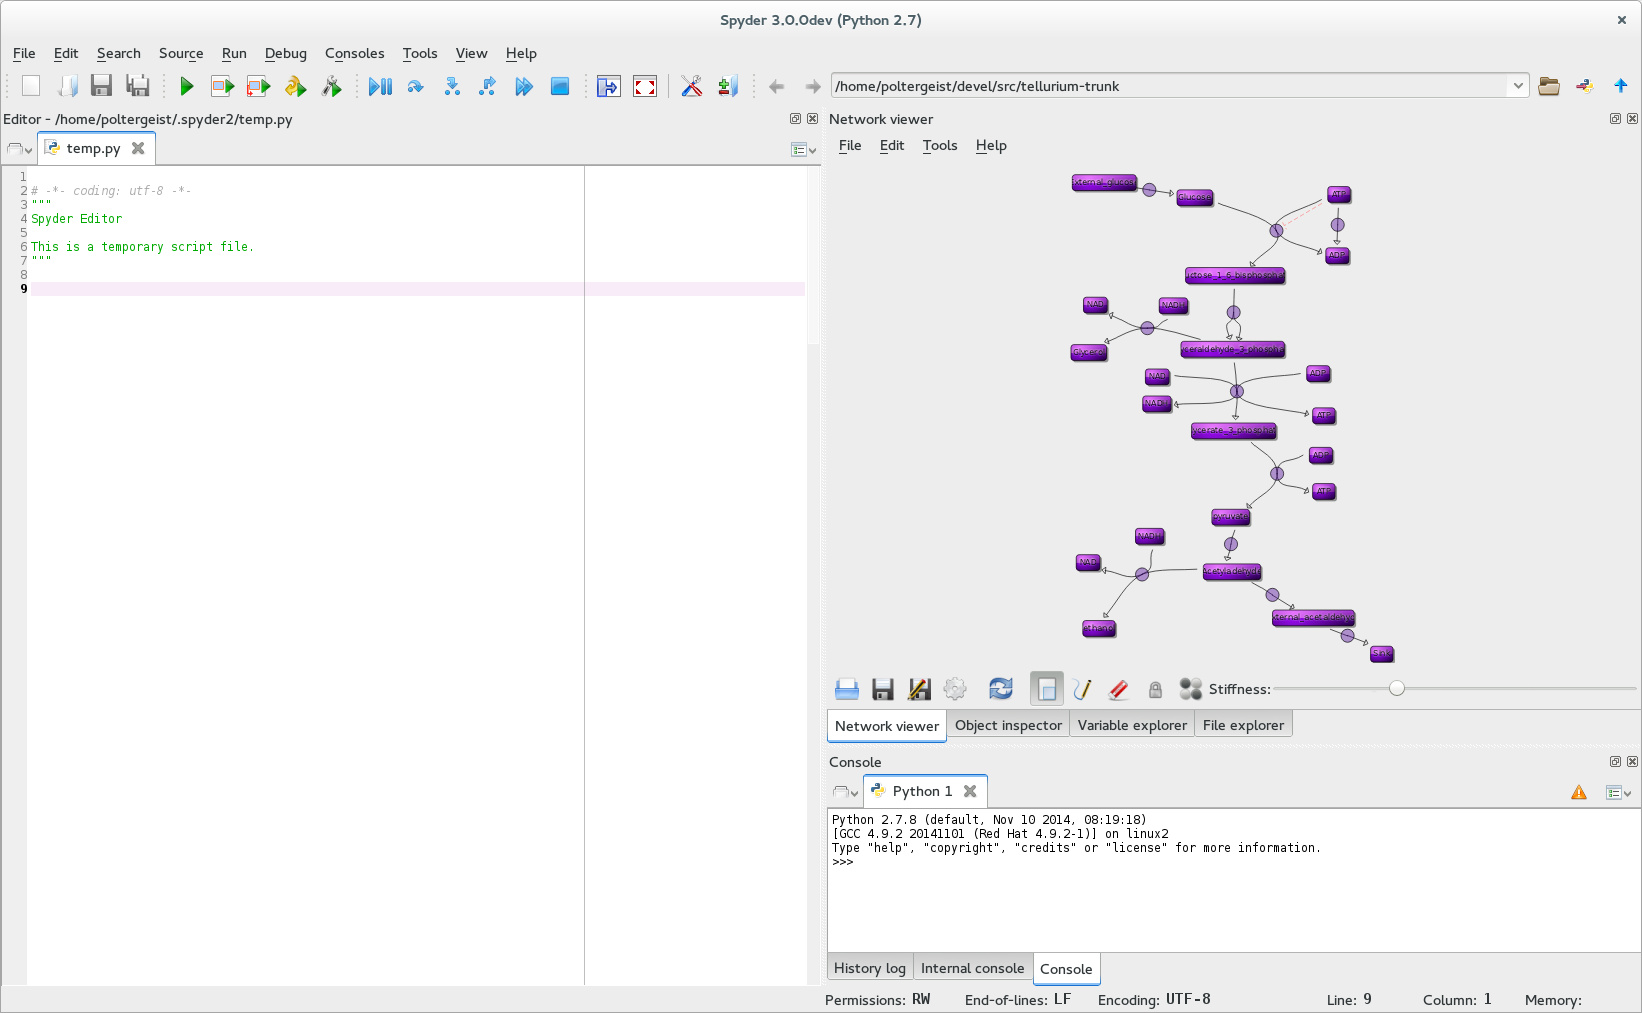
\includegraphics[width=0.3\textwidth]{spyder-nwview-janawolf.jpg}}
  \label{fig:a}
}

\subfigure[A rendered version of the model displayed above]{%
  \centerline{%
  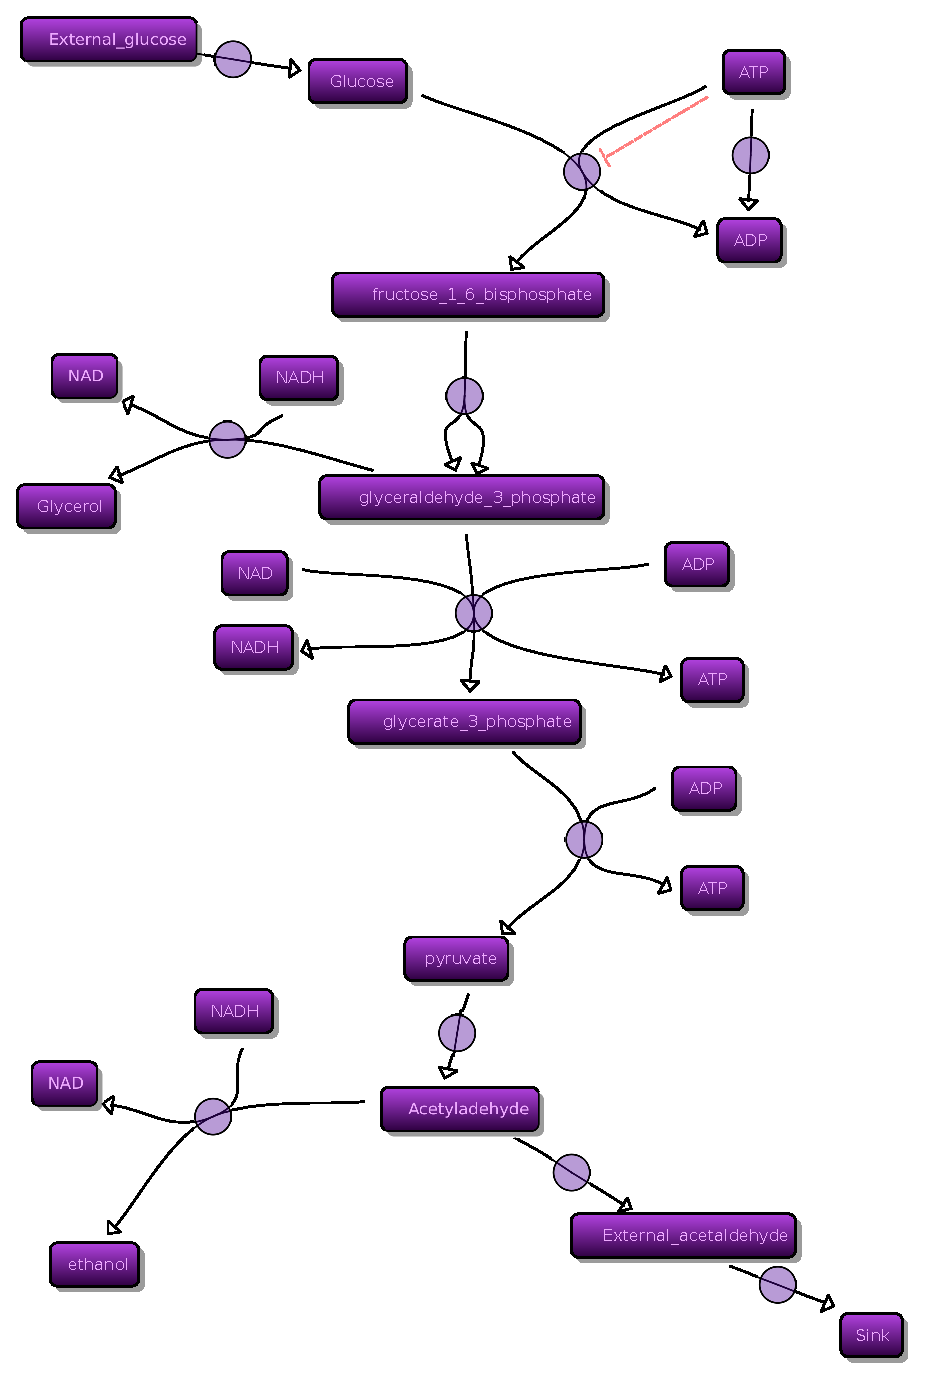
\includegraphics[width=0.30\textwidth]{pyfab-jana-wolf-vector.eps}}
  \label{fig:b}
}

\subfigure[MAPK signaling cascade~\citep{Boris}]{%
  \centerline{%
  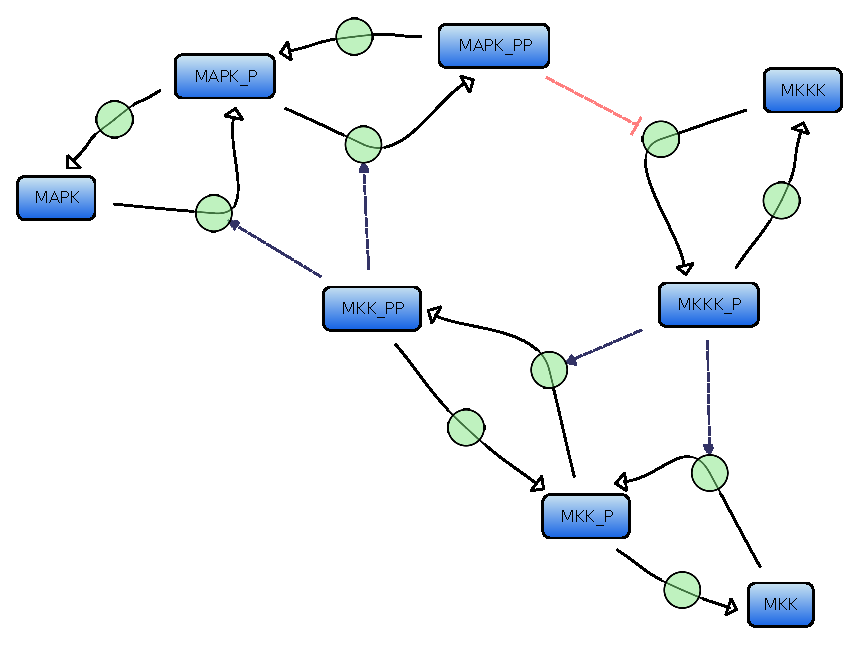
\includegraphics[width=0.30\textwidth]{pyfab-boris-vector.eps}}
  \label{fig:c}
}
\caption{Demonstration of the Python-based network viewer}

\label{fig:01}
\end{figure}

\section{Methods}

\paragraph{SBML Layout Extension Support} 
The library is designed for compatibility across SBML level 2/3, and uses libSBML for reading and writing content~\citep{BornsteinLibSBML2008}. The SBML layout extension is used to store visual layout information. If the input model does not have a layout, one can be automatically generated by the library.

\paragraph{Autolayout Algorithm}
The library automatically generates layout information encoding node and reaction centroid coordinates using the Fruch\-terman-Reingold (FR) algorithm, which has been shown to be robust in the face of variegated graph topologies and faithfully reproduces the underlying symm\-etry~\citep{FruchtermanReingold}. 

\paragraph{Selectively lock Nodes} Users can specify one or more nodes to be locked when the layout algorithm is executed. This ensures that the positions of these nodes do not change when the layout algorithm is applied.
_Node locking is particularly useful for users who want to fine-tune the automatic layout process.

\paragraph{Support for Alias Nodes}
Models with a high degree of connectivity can be problematic for visualization
methods due to the overlap between edges that occurs when the underlying 
graph is embedded in 2D space.
We solve this problem by providing the user
with the ability to create \textit{alias nodes}. In general, any node of degree
$n$ can be decomposed into $n$ alias nodes, each of which is rendered separately.
Using this method, we can reduce the connectivity of any network graph.
The FR-algorithm is particularly adept at laying out such reduced graphs without overlapping edges~\citep{FruchtermanReingold}, 
enabling lucid visualization of complex networks.

\paragraph{Export of Rendered Model}
A rendered model may be exported to a raster format (Portable Network Graphics) or one of several vector formats (Scalable Vector Graphics, TikZ). 

\paragraph{Supply Ancillary graphical Information}
Visual features such as arrowheads/endcaps are supplied by the library, and may be used to render network diagrams as shown in Figure \ref{fig:01}. Five endcap styles are supported and are tied to species roles in SBML reactions: Substrate, product, modifier, activator and inhibitor. 

\paragraph{Language Bindings}
Public APIs for C and Python are provided.
For example, the following Python code loads
an SBML model, applies the FR autolayout algorithm to the network, and saves the result as \texttt{output.xml} in the current directory:

\medskip
\noindent

\begin{lstlisting}[language=python]
# import the sbnw Python module
import sbnw
# load the model
model = sbnw.loadsbml('model.xml')
# seed node coordinates randomly
model.network.randomize()
# apply the FR-algorithm
model.network.autolayout()
# Save new SBML to file
model.save('output.xml')
\end{lstlisting}

\section{Results}

We have deployed libSBNW in the context of the Tellurium biological modeling environment (\href{http://tellurium.analogmachine.org/}{http://tellurium.analog\-mach\-ine.org/}) using the Tellurium's Spyder-based plugin architecture.
Tellurium includes the \texttt{nwed} (network editor) Python module, which may be used to communicate with the layout plugin, and
the SBML model may be set or retrieved via \texttt{nwed.setsbml} and
\texttt{nwed.getsbml} respectively.
%
\begin{lstlisting}[language=python]
sbmlStr = '''...'''
import nwed
nwed.setsbml(sbmlSstr)
\end{lstlisting}

\section*{Acknowledgments}
We acknowledge Stanley Gu for his shared web development expertise, Lucian Smith for his work on the Antimony language, Jonathan Gallimore for his work on the C API, Andy Somogyi for his shared expertise in Python extension modules, and Kaylene Stocking for testing the network viewer.

\paragraph{Funding\textcolon} The authors are most grateful to generous funding from the National Institute of General Medical Sciences of the National Institutes of Health under award R01-GM081070. The content is solely the responsibility of the authors and does not necessarily represent the official views of the National Institutes of Health.

% suppress bib numbers
\makeatletter
\renewcommand\@biblabel[1]{}
\makeatother

\begin{thebibliography}{}

\bibitem[Berg\-man and Sauro, 2006]{BergmanSBW2006} Bergmann, F. T., and Sauro, H. M. (2006) SBW-a modular framework for systems biology, {\it Proceedings of the 38th conference on Winter simulation}, 1637--1645.

\bibitem[Bornstein {\it et~al}., 2008]{BornsteinLibSBML2008} Bornstein, B, Keating, S, Jouraku, A, and Hucka (2008) LibSBML: an API Library for SBML, {\it Bioinformatics}, {\bf 24} 6, 880--881.

\bibitem[Deckard {et~al}., 2006]{Deckard2006} Deckard, A, Bergmann, F.T and Sauro H.M. (2006) Supporting the SBML layout extension, {\it Bioinformatics} {\bf 22} 23 2966--2967.

\bibitem[Dr\"{a}ger {et~al}., 2014]{Drager2014} Dr\"{a}ger, A and Palsson B (2014) Improving Collaboration by Standardization Efforts in Systems Biology, {\it Frontiers in Bioengineering and Biotechnology} {\bf 2} 61.

\bibitem[Fruchterman and Reingold, 1991]{FruchtermanReingold} Fruchterman, T.M.J. and Reingold, E.M. (1991) Graph drawing by force-directed placement, {\it Software: Practice and Experience}, {\bf 21} 11, 1129--1164.

\bibitem[Gauges {et~al}., 2006]{Gauges2006} Gauges, R, {\it et~al} (2006) A model diagram layout extension for SBML, {\it Bioinformatics} {\bf 22} 15 1879-1885.

\bibitem[Gauges, 2009]{Gauges2009} Gauges, R (2009) Complementing layout information with render information in SBML files.  University of Heidelberg. Available at \href{http://otto.bioquant.uni-heidelberg.de/sbml/level2/20091029/SBMLRenderExtension-20091029.pdf}{http://otto.bioquant.uni-heidelberg.de/sbml/level2/20091029/SBMLRenderExtension-20091029.pdf}

\bibitem[Hucka {et~al}., 2003]{Hucka:2003fs} Hucka, M, Finney, A, Sauro, H.M, Bolouri, H, Doyle, J, Kitano, H and
  the rest of~the SBML~Forum. The systems biology markup language (SBML): a medium for representation and exchange of biochemical network models.{\em Bioinformatics\/}, {\bf 19}(4), 524--531.

\bibitem[Kholodenko, 2000]{Boris} Kholodenko, B. N. (2000) Negative feedback and ultrasensitivity can bring about oscillations in the mitogen-activated protein kinase cascades, {\it European journal of biochemistry / FEBS}, {\bf 267} 6, 1583--1588.

\bibitem[Sauro, 2014]{Sauro2014} Sauro H. M. (2014) Systems Biology: An Introduction to Pathway Modeling, Ambrosius Publishing, ISBN-10: 0982477376

\bibitem[Wolf and Heinrich, 2000]{WolfGlyco2000} Wolf, J and Reinhart H (2000) Effect of cellular interaction on glycolytic oscillations in yeast: a theoretical investigation, {\it Biochemical Journal}, {\bf 345}, 321--334.

% not used in text
%\bibitem[Zhao {\it et~al}., 2011]{Zhao2011} Zhao, T, Wang, D, Hong and Hoon (2011) Solution formulas for cubic equations without or with constraints, {\it Journal of Symbolic Computation}, {\bf 46} 8, 904--918.


% \bibitem[Bofelli {\it et~al}., 2000]{Boffelli03} Bofelli,F., Name2, Name3 (2003) Article title, {\it Journal Name}, {\bf 199}, 133-154.

% \bibitem[Bag {\it et~al}., 2001]{Bag01} Bag,M., Name2, Name3 (2001) Article title, {\it Journal Name}, {\bf 99}, 33-54.

% \bibitem[Yoo \textit{et~al}., 2003]{Yoo03}
% Yoo,M.S. \textit{et~al}. (2003) Oxidative stress regulated genes
% in nigral dopaminergic neurnol cell: correlation with the known
% pathology in Parkinson's disease. \textit{Brain Res. Mol. Brain
% Res.}, \textbf{110}(Suppl. 1), 76--84.

% \bibitem[Lehmann, 1986]{Leh86}
% Lehmann,E.L. (1986) Chapter title. \textit{Book Title}. Vol.~1, 2nd edn. Springer-Verlag, New York.

% \bibitem[Crenshaw and Jones, 2003]{Cre03}
% Crenshaw, B.,III, and Jones, W.B.,Jr (2003) The future of clinical
% cancer management: one tumor, one chip. \textit{Bioinformatics},
% doi:10.1093/bioinformatics/btn000.

% \bibitem[Auhtor \textit{et~al}. (2000)]{Aut00}
% Auhtor,A.B. \textit{et~al}. (2000) Chapter title. In Smith, A.C.
% (ed.), \textit{Book Title}, 2nd edn. Publisher, Location, Vol. 1, pp.
% ???--???.

% \bibitem[Bardet, 1920]{Bar20}
% Bardet, G. (1920) Sur un syndrome d'obesite infantile avec
% polydactylie et retinite pigmentaire (contribution a l'etude des
% formes cliniques de l'obesite hypophysaire). PhD Thesis, name of
% institution, Paris, France.

\end{thebibliography}
\end{document}
